\documentclass[11pt,a4paper]{article}

\usepackage[utf8]{inputenc}
\usepackage[T1]{fontenc}
\usepackage{amsmath}
\usepackage{graphicx}
\usepackage{hyperref}
\usepackage{booktabs}
\usepackage{tabularx}
\usepackage{array}
\usepackage{tikz}
\usetikzlibrary{arrows.meta, positioning}

\title{Bilingual English--Romanian Text Summarization}
\author{Buian Dragos}

\begin{document}
\maketitle

% ---------------------------------------------------------------------------
\section{Problem statement}
% ---------------------------------------------------------------------------

Abstractive text summarization produces a short summary that captures the main ideas of a longer document.
In this project we address \textbf{bilingual summarization} for \textbf{English (EN)} and \textbf{Romanian (RO)}: given a source article, the system must generate a concise summary in the same language.

The task is challenging because:
\begin{itemize}
  \item summaries must be fluent and informative (semantic quality);
  \item generated text should remain faithful to the source (factual consistency);
  \item a single multilingual model must handle both languages and multiple dataset formats.
\end{itemize}

% ---------------------------------------------------------------------------
\section{Proposed solution}
% ---------------------------------------------------------------------------

\subsection{Theoretical aspects}

We treat summarization as \textbf{sequence-to-sequence (seq2seq) learning}.
Let $x = (x_1, \ldots, x_n)$ be the tokenized source document and $y = (y_1, \ldots, y_m)$ the reference summary.
The model learns parameters $\theta$ that maximize the conditional likelihood:
\[
  \mathcal{L}(\theta) = \sum_{(x,y) \in \mathcal{D}} \log P_\theta(y \mid x)
  = \sum_{(x,y) \in \mathcal{D}} \sum_{t=1}^{m} \log P_\theta(y_t \mid y_{<t}, x).
\]

We fine-tune \textbf{mT5} (\texttt{google/mt5-small}), a multilingual T5 encoder--decoder, on a mixed EN+RO training set.
At inference time we use \textbf{beam search} (beam width $B=4$) to approximate
\[
  \hat{y} = \arg\max_{y} P_\theta(y \mid x).
\]

\textbf{Semantic quality} is measured with \textbf{BERTScore} (contextual embedding similarity between prediction and reference).
\textbf{Factual consistency} is measured with \textbf{SummaC}, which scores whether the summary is supported by the source.

\subsection{Data sets used in the application}

All corpora are loaded via Hugging Face \texttt{datasets} and normalized to a common schema:
\texttt{id}, \texttt{language}, \texttt{dataset}, \texttt{source}, \texttt{reference}.
If a corpus lacks \texttt{validation} or \texttt{test}, splits are created automatically (e.g.\ 80/10/10 from train).

\begin{table}[htbp]
  \centering
  \small
  \caption{Corpora used in the pipeline.}
  \label{tab:datasets}
  \setlength{\tabcolsep}{5pt}
  \renewcommand{\arraystretch}{1.15}
  \begin{tabularx}{\linewidth}{@{}>{\raggedright\arraybackslash}p{0.5cm} >{\raggedright\arraybackslash}p{2.1cm} X@{}}
    \toprule
    & Dataset & Hugging Face id and field mapping \\
    \midrule
    EN & CNN/DailyMail &
      \nolinkurl{cnn_dailymail} \\
    & & article $\rightarrow$ source, highlights $\rightarrow$ reference \\
    \addlinespace
    EN & XSum &
      \nolinkurl{xsum} \\
    & & document $\rightarrow$ source, summary $\rightarrow$ reference \\
    \addlinespace
    RO & ReaderBench &
      \nolinkurl{readerbench/ro-text-summarization} \\
    & & Content $\rightarrow$ source, Summary $\rightarrow$ reference \\
    \addlinespace
    RO & MassiveSumm &
      \nolinkurl{MaLA-LM/MassiveSumm_long} (language \texttt{ron}) \\
    & & text $\rightarrow$ source, summary $\rightarrow$ reference \\
    \bottomrule
  \end{tabularx}
\end{table}

Training, validation, and test examples from all selected datasets are \textbf{concatenated and shuffled} (with optional per-dataset caps for smoke runs).

\subsection{Application}

The application is a command-line \textbf{pipeline} with stages: prepare $\rightarrow$ train $\rightarrow$ infer $\rightarrow$ eval (optional smoke test).

\begin{figure}[h]
  \centering
  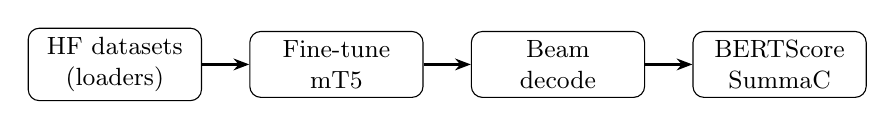
\begin{tikzpicture}[
    node distance=1.1cm and 0.6cm,
    box/.style={draw, rounded corners, minimum width=2.2cm, minimum height=0.7cm, align=center, font=\small},
    arr/.style={-{Stealth[length=2mm]}, thick}
  ]
    \node[box] (data) {HF datasets\\(loaders)};
    \node[box, right=of data] (train) {Fine-tune\\mT5};
    \node[box, right=of train] (infer) {Beam\\decode};
    \node[box, right=of infer] (eval) {BERTScore\\SummaC};
    \draw[arr] (data) -- (train);
    \draw[arr] (train) -- (infer);
    \draw[arr] (infer) -- (eval);
  \end{tikzpicture}
  \caption{End-to-end workflow (\texttt{python -m src.pipeline}).}
\end{figure}

Outputs are written under \texttt{practical/outputs/}: checkpoints, JSONL predictions, and JSON/CSV evaluation reports.

% ---------------------------------------------------------------------------
\section{Implementation --- details}
% ---------------------------------------------------------------------------

\subsection{Project layout}

\begin{verbatim}
practical/
  src/
    config.py          # paths, model names, lengths, seed
    pipeline.py        # orchestrates stages
    train.py           # Seq2SeqTrainer fine-tuning
    infer.py           # batch generation
    data/loaders.py    # dataset load + normalize + merge
    eval/
      bertscore_eval.py
      summac_eval.py
  outputs/             # checkpoints, predictions, reports
\end{verbatim}

\subsection{Libraries and main APIs}

\begin{itemize}
  \item \textbf{PyTorch / Hugging Face Transformers} --- \texttt{AutoModelForSeq2SeqLM}, \texttt{AutoTokenizer}, \texttt{Seq2SeqTrainer}, \texttt{Seq2SeqTrainingArguments}, \texttt{DataCollatorForSeq2Seq}.
  \item \textbf{Hugging Face Datasets} --- \texttt{load\_dataset}, \texttt{concatenate\_datasets}, split helpers in \texttt{src/data/loaders.py}.
  \item \textbf{bert-score} --- multilingual BERTScore (\texttt{xlm-roberta-large} by default).
  \item \textbf{SummaC} --- factual consistency scoring on (source, prediction) pairs.
  \item \textbf{accelerate} --- training backend used by Transformers.
\end{itemize}

\subsection{Key functions and entry points}

\begin{itemize}
  \item \texttt{load\_all\_datasets}, \texttt{build\_combined\_split} --- load EN/RO corpora and build mixed splits.
  \item \texttt{tokenize\_dataset} --- encode sources and summary labels for training.
  \item \texttt{src.train} --- fine-tune and save checkpoint to \texttt{outputs/checkpoints/mt5-small-en-ro}.
  \item \texttt{src.infer} --- write \texttt{test\_predictions.jsonl}.
  \item \texttt{src.eval.bertscore\_eval}, \texttt{src.eval.summac\_eval} --- produce report files.
  \item \texttt{src.pipeline} --- run selected stages from one CLI.
\end{itemize}

\subsection{Default hyperparameters}

\begin{center}
\small
\begin{tabular}{@{}ll@{}}
  \toprule
  Setting & Value \\
  \midrule
  Base model & \texttt{google/mt5-small} \\
  Max source / target length & 512 / 128 \\
  Learning rate & $5 \times 10^{-5}$ \\
  Beam size (inference) & 4 \\
  Random seed & 42 \\
  \bottomrule
\end{tabular}
\end{center}

% ---------------------------------------------------------------------------
\section{Experiments and results}
% ---------------------------------------------------------------------------

\subsection{Experimental setup}

All runs were executed on a workstation with an \textbf{NVIDIA GeForce GTX~1070} (8\,GB VRAM), using the conda environment defined in \texttt{environment.yml}.
We use \texttt{google/mt5-small} rather than \texttt{mt5-base} to fit GPU memory and reduce training time.
Table~\ref{tab:exp-setup} summarizes the pilot experiment reported below.

\begin{table}[h]
  \centering
  \small
  \caption{Pilot training and evaluation configuration.}
  \label{tab:exp-setup}
  \begin{tabularx}{\textwidth}{@{}l X@{}}
    \toprule
    Setting & Value \\
    \midrule
    Model & \texttt{google/mt5-small} \\
    EN datasets & CNN/DailyMail, XSum \\
    RO datasets & ReaderBench, MassiveSumm (\texttt{ron}) \\
    Cap per dataset & 2\,000 (train / val / test) \\
    Epochs & 1 \\
    Batch size (train / eval) & 2 / 2 \\
    Max source / target length & 512 / 128 \\
    Optimizer & AdamW, lr $=5\times10^{-5}$, warmup 0.05 \\
    Inference & beam search ($B=4$) \\
    Metrics & BERTScore (\texttt{xlm-roberta-large}), SummaC (\texttt{vitc}) \\
    Checkpoint & \texttt{outputs/checkpoints/mt5-small-en-ro} \\
    \bottomrule
  \end{tabularx}
\end{table}

Training consumed ${\sim}$6\,000 mixed examples (${\sim}$3\,000 optimization steps) and completed in ${\sim}$18 minutes on the target GPU.
The final training loss was $5.05$; validation loss after one epoch was $2.86$.
Inference on the combined test split produced \textbf{6\,000} predictions: 2\,000 per corpus (CNN/DailyMail, XSum, ReaderBench).

\subsection{Semantic quality (BERTScore)}

BERTScore F1 was computed on all 6\,000 test predictions against the reference summaries.
Table~\ref{tab:bertscore} reports mean F1 by language and dataset.

\begin{table}[h]
  \centering
  \small
  \caption{BERTScore F1 on the test split ($n=6\,000$).}
  \label{tab:bertscore}
  \begin{tabular}{@{}llrr@{}}
    \toprule
    Lang. & Dataset & $n$ & F1 \\
    \midrule
    EN & CNN/DailyMail & 2\,000 & 0.878 \\
    EN & XSum & 2\,000 & 0.874 \\
    RO & ReaderBench & 2\,000 & 0.875 \\
    \midrule
    \multicolumn{2}{l}{Macro-average} & & 0.875 \\
    \bottomrule
  \end{tabular}
\end{table}

Scores are high and stable across languages (${\sim}$0.87--0.88), indicating that the generated summaries are semantically close to the references under this shallow fine-tuning regime.
This is expected partly because mT5-small is pretrained and the evaluation set overlaps the fine-tuning distribution; stronger gains would require longer training or full-corpus fine-tuning.

\subsection{Factual consistency (SummaC)}

SummaC is substantially slower than BERTScore on long news articles, so we first evaluated a \textbf{random 200-example subset} of the prediction file (\texttt{summac\_report\_200.json}).
Table~\ref{tab:summac} lists mean SummaC scores and the fraction of summaries marked factual at threshold~0.5.

\begin{table}[h]
  \centering
  \small
  \caption{SummaC on a 200-example test subset (threshold $=0.5$).}
  \label{tab:summac}
  \begin{tabular}{@{}llrr@{}}
    \toprule
    Lang. & Dataset & $n$ & Mean score \\
    \midrule
    EN & CNN/DailyMail & 58 & $-0.107$ \\
    EN & XSum & 66 & $-0.095$ \\
    RO & ReaderBench & 76 & $0.282$ \\
    \bottomrule
  \end{tabular}
\end{table}

\noindent
On this subset, \textbf{25\%} of summaries exceeded the factuality threshold (score $\geq 0.5$).
English news domains (CNN/DailyMail, XSum) received negative mean SummaC scores, while Romanian ReaderBench summaries scored higher on average.
This pattern suggests that semantic overlap with references (BERTScore) does not imply source faithfulness: the model can produce fluent text that is poorly supported by the source, especially on abstractive English headlines.

\subsection{Discussion and next steps}

The pilot run validates the full pipeline (load $\rightarrow$ train $\rightarrow$ infer $\rightarrow$ eval) on bilingual data with practical resource constraints.
Limitations of this experiment include: (i)~only one epoch on capped subsets, (ii)~a smaller encoder (\texttt{mt5-small}), and (iii)~partial SummaC evaluation due to runtime.
Promising follow-ups are full-corpus fine-tuning, mixed-precision training on GPU, faster greedy decoding for development, and completing SummaC on the full 6\,000-example test set.

\end{document}
